\newpage


\subsubsection{UCA 5 - Visualizzazione dello storico accessi presso un'organizzazione}
\begin{figure}[h]
	\centering	
	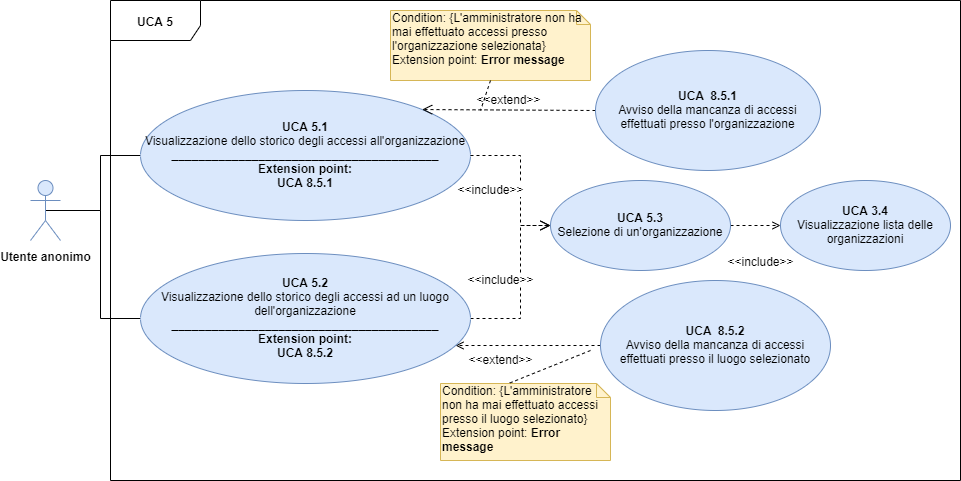
\includegraphics[scale=0.5]{sezioni/UseCase/Immagini/UCA5.png}
	\caption{UCA 5 - Visualizzazione dello storico accessi presso un'organizzazione}
\end{figure}

\begin{itemize}
    \item \textbf{Attori primari:} Utente autenticato;
    %\item \textbf{Attori secondari:}%opzionale
    \item \textbf{Precondizione:} L'utente ha precedentemente aggiunto l'organizzazione di cui vuole visualizzare i propri accessi alla lista delle organizzazione preferite;
    \item \textbf{Postcondizione:} L'utente visualizza nella schermata dell'applicazione la lista degli accessi effettuati presso i luoghi dell'organizzazione (con nome del luogo, timestamp di ingresso, di uscita, e tempo di permanenza);
    Se si trova all'interno di un luogo viene visualizzato il tempo passato al suo interno fino a quel momento;
    \item \textbf{Scenario principale:} L'utente può visualizzare la lista dei propri accessi presso un'organizzazione, se questa non è vuota, altrimenti premia la selezione di un'organizzazione fra quelle presenti nella lista delle preferite dall'utente; %forse si può frammentare e metterla come caso d'uso separato, tipo come eccezzione 
    %\item \textbf{Estensioni:}
    \item \textbf{Estensioni:}
    \begin{enumerate}
        \item UCA 3.3.3 - Visualizzazione di un messaggio di errore che informa che non è salvata nessuna lista delle organizzazioni;	
    \end{enumerate}	
    \item \textbf{Inclusioni:}
    \begin{itemize}
        \item UCA 5.1 - Visualizzazione della lista delle organizzazioni preferite;
        \item UCA 5.2 - Visualizzazione della lista degli accessi presso un'organizzazione.
    \end{itemize}

\end{itemize}


\subsubsection{UCA 5.1 - Visualizzazione della lista delle organizzazioni preferite}
\begin{itemize}
    \item \textbf{Attori primari:} Utente autenticato;
    %\item \textbf{Attori secondari:}%opzionale
    \item \textbf{Precondizione:} L'utente ha precedentemente aggiunto le organizzazioni da visualizzare nella lista delle organizzazioni preferite;
    \item \textbf{Postcondizione:} L'utente visualizza nella schermata dell'applicazione la lista delle proprie organizzazioni preferite; 
    \item \textbf{Scenario principale:} L'utente vuole visualizzare la lista delle proprie organizzazioni preferite; %, se questa non è vuota, e da qui procedere con UCA 5.2.
    %\item \textbf{Scenario alternativo:} L'utente non ha organizzazioni preferite, per cui viene visualizzato un avviso come indicato in UCA 5.1.1.
    \item \textbf{Flusso di eventi:}
    \begin{enumerate}
        \item L'utente seleziona la funzionalità "Storico accessi";
    \end{enumerate}
    \item \textbf{Estensioni:}
    \begin{itemize}
        \item UCA 5.1.1 - Avviso di assenza di organizzazioni preferite.
    \end{itemize}
    %\item \textbf{Inclusioni:}
\end{itemize}

\subsubsection{UCA 5.1.1 - Avviso di assenza di organizzazioni preferite}
\begin{itemize}
    \item \textbf{Attori primari:} Utente autenticato;
    %\item \textbf{Attori secondari:}%opzionale
    \item \textbf{Precondizione:} L'utente non ha aggiunto alcuna organizzazione come preferita;
    \item \textbf{Postcondizione:} L'utente visualizza nella schermata un messaggio che lo avvisa della mancanza di organizzazioni.
\end{itemize}

\subsubsection{UCA 5.2 - Visualizzazione della lista degli accessi presso un'organizzazione}
\begin{itemize}
    \item \textbf{Attori primari:} Utente autenticato;
    %\item \textbf{Attori secondari:}%opzionale
    \item \textbf{Precondizione:} L'utente ha selezionato dalla lista delle organizzazioni preferite un'organizzazione di cui visualizzare i propri accessi;
    \item \textbf{Postcondizione:} L'utente visualizza nella schermata dell'applicazione la lista degli accessi effettuati presso i luoghi dell'organizzazione (con descrizione del luogo, timestamp di ingresso, di uscita, e tempo di permanenza).
    Se si trova all'interno di un luogo viene visualizzato il tempo passato al suo interno fino a quel momento;
    \item \textbf{Scenario principale:} L'utente può visualizzare tutti gli accessi da lui fatti presso i luoghi dell'organizzazione, in modalità di tracciamento anonimo e autenticato;
    \item \textbf{Scenario alternativo:} L'utente ha effettuato l'accesso presso il luogo dell'organizzazione ma non ne è ancora uscito. In questo caso, viene visualizzato un timer con il tempo trascorso dal momento in cui è entrato.
    Una volta uscito dal luogo, vale il comportamento descritto nello scenario principale;
    \item \textbf{Flusso di eventi:}
    \begin{enumerate}
        \item UCA 5.1 - Visualizzazione della lista delle organizzazioni;
        \item L'utente, per precondizione, ha selezionato un'organizzazione di cui visualizzare i propri accessi nei suoi luoghi; %----> renderlo un UCA oppure sistemarlo
    \end{enumerate}
    \item \textbf{Estensioni:}
    \begin{itemize}
        \item UCA 5.2.1 - Avviso di assenza di accessi presso i luoghi di un'organizzazione.
    \end{itemize}
    %\item \textbf{Inclusioni:}
\end{itemize}

\subsubsection{UCA 5.2.1 - Avviso di assenza di accessi presso i luoghi di un'organizzazione}
\begin{itemize}
    \item \textbf{Attori primari:} Utente autenticato;
    %\item \textbf{Attori secondari:}%opzionale
    \item \textbf{Precondizione:} L'utente ha selezionato dalla lista delle organizzazioni preferite un'organizzazione di cui visualizzare i propri accessi, ma non ha mai effettuato accesso ai luoghi dell'organizzazione;
    %L'utente seleziona un organizzazione di cui non dispone di alcun accesso
    \item \textbf{Postcondizione:} L'utente visualizza nella schermata un messaggio che lo avvisa della mancanza di accessi nei luoghi dell'organizzazione.
\end{itemize}

% \begin{figure}[h]
% 	\centering
% 	
% 	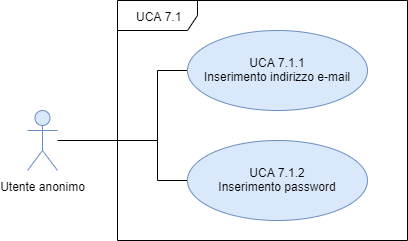
\includegraphics[scale=0.5]{sezioni/UseCase/Immagini/UCA7.1.png}
%	\caption{UCA 6.1 - Ordinamento della lista degli accessi presso un’organizzazione}
% \end{figure}
\subsubsection{UCA 5.2.2 - Ordinamento per data decrescente della lista degli accessi}
\begin{itemize}
    \item \textbf{Attori primari:} Utente autenticato;
    %\item \textbf{Attori secondari:}%opzionale
    \item \textbf{Precondizione:} L'utente ha a disposizione una lista di accessi presso uno o più luoghi di un organizzazione preferita;
    \item \textbf{Postcondizione:} L'utente ottiene la lista di accessi iniziale riordinata in ordine decrescente.
%    \item \textbf{Flusso di eventi:}
%    \begin{enumerate}
%        \item UCA 5.2 - Visualizzazione della lista degli accessi presso un'organizzazione;
%        \item L'utente seleziona la funzionalità "Ordinamento lista accessi".
%        \item L'utente sceglie la funzionalità "Ordinamento per data (decrescente)".
%    \end{enumerate}
\end{itemize}

\subsubsection{UCA 5.2.3 - Ordinamento per data crescente della lista degli accessi}
\begin{itemize}
    \item \textbf{Attori primari:} Utente autenticato;
    %\item \textbf{Attori secondari:}%opzionale
    \item \textbf{Precondizione:} L'utente ha a disposizione una lista di accessi presso uno o più luoghi di un organizzazione preferita;
    \item \textbf{Postcondizione:} L'utente ottiene la lista di accessi iniziale riordinata in ordine crescente (ovvero una data meno recente è considerata più piccola di una data più recente).
%    \item \textbf{Inclusioni:} % non sono sicuro sia corretto
%    \begin{itemize}
%        \item UCA 5.2 - Visualizzazione della lista degli accessi presso un'organizzazione.
%    \end{itemize}
%    \item \textbf{Flusso di eventi:}
%    \begin{enumerate}
%        \item L'utente esegue il caso d'uso UCA 5.2
%        \item l'utente seleziona la funzionalità "Ordinamento lista accessi".
%        \item l'utente sceglie la funzionalità "Ordinamento per data (crescente)".
%    \end{enumerate}
\end{itemize}

\subsubsection{UCA 5.2.4 - Filtro per luogo della lista degli accessi presso un'organizzazione}
\begin{itemize}
    \item \textbf{Attori primari:} Utente Riconosciuto, Utente Anonimo.
    \item \textbf{Precondizione:} L'utente ha a disposizione una lista di accessi presso uno o più luoghi di un organizzazione preferita.
    \item \textbf{Precondizione:} L'utente ottiene la lista di accessi iniziale presso un singolo luogo selezionato.
%    \item \textbf{Inclusioni:} % non sono sicuro sia corretto
%    \begin{itemize}
%        \item UCA 5.2 - Visualizzazione della lista degli accessi presso un'organizzazione.
%    \end{itemize}
%    \item \textbf{Flusso di eventi:}
%    \begin{enumerate}
%        \item L'utente esegue il caso d'uso UCA 5.2
%        \item l’utente seleziona la funzionalità “Filtro per luogo”.
%        \item l’utente seleziona un luogo dell’organizzazione di cui mostrare gli accessi.
%    \end{enumerate}
\end{itemize}